\documentclass[11pt]{article}
\usepackage{graphicx}
\usepackage{hyperref}
\usepackage{natbib}

\setlength{\textwidth}{6.5in}
\setlength{\headheight}{0in}
\setlength{\textheight}{8.0in}
\setlength{\hoffset}{0in}
\setlength{\voffset}{0in}
\setlength{\oddsidemargin}{0in}
\setlength{\evensidemargin}{0in}

\title{Example report file}
  
\author{Michael R. Blanton}


\begin{document}

\maketitle

\abstract{This document has an outline of a report with figures, with
 the sections that your report should contain. The abstract should
 have a paragraph encapsulation of the motivation, methods, and major
 results of the report.}

\section{Introduction}
\label{sec:intro}

The introduction should give motivation and background material for
the project. It should not be overly long, so the background material
should only be what is necessary to support the motivation for the
project.

The background material (or later parts of the text) may refer to
references which the reader can pursue. The
\href{http://www.bibtex.org}{BibTeX} system is ideal for tracking
references. The author of this course's book (\citealt{newman2012a})
has also written many scientific articles, for example
\citet{newman2002a}.

The introduction should end with a short outline of the paper. In the
following sections we will describe what a methods section should
contain (\S\ref{sec:methods}), 

\section{Methods}
\label{sec:methods}

This section should contain the problem description, any preliminary
analysis necessary to help set up the computational problem, and how
you did the computation. This section may be fairly long and can be
broken into subsections (as may other sections). You should use your
judgment about how to organize this section for readability.

\subsection{Formulation of the problem}
\label{sec:formulation}

For example, one section might describe how to write the problem in a
mathematically convenient form.

\subsection{Computational methods}
\label{sec:computational}

Another section might describe the specific computational methods.

\section{Results}
\label{sec:results}

This section should contain the results. If appropriate, it should
start with test cases with known solutions or other validation tests
for the methods. Then it should go on to show the results of your
analysis for the more interesting cases.

The discussion in this section is best if it is fairly minimal. ``Just
the facts'' is good place to start. Sometimes it is useful however to
impose some narrative flow; i.e. describe why each case is important
to look at.

It can be difficult to judge what is appropriate to put in the
report. You should begin by being very inclusive regarding the results
you should.

This section should definitely have figures (e.g. Figure
\ref{fig:example}), though they may be appropriate in other sections
too.

\begin{figure}[b!]
\centering
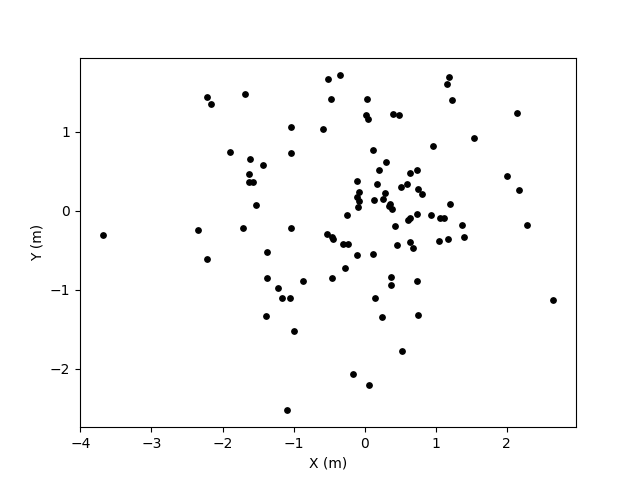
\includegraphics[width=0.95\textwidth]{scatter.png}
\caption{ \label{fig:example} This is just an example. Notice that
  both axes of the figure are labeled, and the units are given.}
\end{figure}
  
\section{Discussion}

The discussion should be where you impose interpretation on the
results. This discussion will have different forms depending on the
goals of the project. What can you conclude about the problem or about
the methods involved? Are you able to reach a conclusion about the
relative merits of different methods? Are these results expected? How
does this work compare with previously determined results? What are
the caveats and limitations of this work?

\bibliographystyle{apj}
\bibliography{example}

\end{document}

 
 
